\section{Dijkstra Algorithm}

\begin{frame}{Dijkstra Algorithm}{Shortest Path without Computer}
  \begin{itemize}
    \item
      Wanted: Shortest path from M to all other points
    \item
      Place pearls on crossings and clamp strings between them
  \end{itemize}
%  \begin{figure}
%    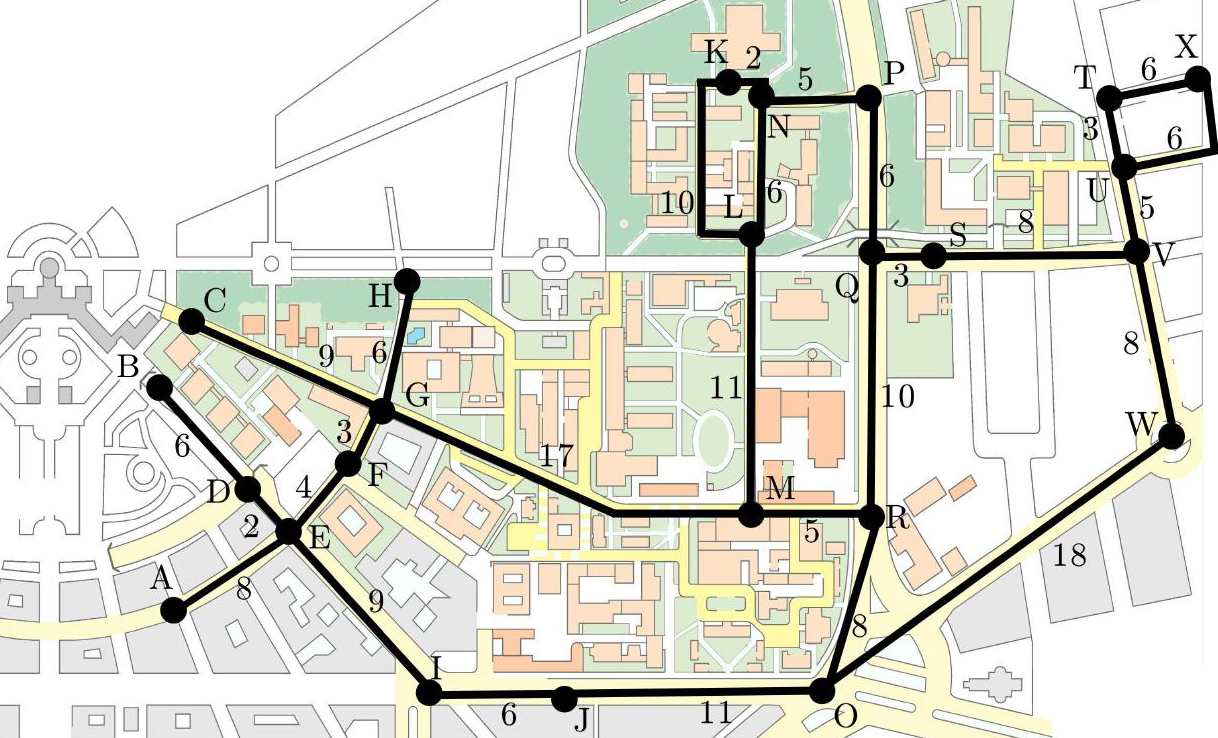
\includegraphics[width=0.75\linewidth]{Images/Dijkstra/DijkstraMap}
%    \caption{Map $\copyright\,$ Mehlhorn / Sanders}
%  \end{figure}
\end{frame}

%-------------------------------------------------------------------------------

\begin{frame}{Dijkstra Algorithm}{Shortest Path without Computer}
  \vspace{-1.5em}
  \begin{columns}
    \begin{column}{0.55\linewidth}
%      \begin{figure}[!t]
%        \includegraphics[width=0.8\linewidth]
%          {Images/Dijkstra/DijkstraMap}
%        \caption{Map $\copyright\,$ Mehlhorn / Sanders}
%      \end{figure}
%      \vspace{-1.5em}
      \begin{itemize}
        \item
          Take the net and pull it slowly upwards until fully lifted
        \item
          Each node (pearl) now has a specific height
        \item
          The distance to M is exactly the {\color{Mittel-Blau}shortest path}
      \end{itemize}
    \end{column}
    \begin{column}{0.45\linewidth}
%      \begin{figure}[!t]
%        \includegraphics[width=\linewidth]
%          {Images/Dijkstra/DijkstraTree_WithOverlay}
%        \vspace{-0.5em}
%        \caption{Map $\copyright\,$ Mehlhorn / Sanders}
%      \end{figure}
    \end{column}
  \end{columns}
\end{frame}

%-------------------------------------------------------------------------------

\begin{frame}{Dijkstra Algorithm}{Shortest Path}
  \vspace{-1.5em}
  \begin{figure}
    \begin{adjustbox}{width=0.75\linewidth}
      \begin{tikzpicture}[
  vertex/.style={
    circle,
    draw=Mittel-Blau,
    color=Mittel-Blau,
    fill=Hell-Blau,
    inner sep=0em,
    minimum size=1.75em,
    line width=0.1em,
    font=\large,
    solid
  }, vertex_shadow/.style={
    vertex,
    draw=black,
    color=black,
    fill=white,
    dotted
  }, edge/.style={
    draw=Mittel-Gruen,
    line width=0.2em
  }, edge_arrow/.style={
    edge,
    ->
  }, edge_label/.style={
    sloped,
    anchor=south,
    auto=false
  }
]%
% Draw vertices
\draw (9.0, 0.0) node[vertex] (end) {$t$};
\draw[edge_arrow, dashdotted]
  (0.0, 0.0) .. controls (3.0, 1.5) and (6.0, 0.0) .. (end.west)
  node[vertex, pos=0.0] {$s$}
  node[vertex, pos=0.2] {$u_1$}
  node[vertex_shadow, pos=0.4] {}
  node[vertex, pos=0.6] {$u_2$}
  node[vertex_shadow, pos=0.8] {}
  node[pos=0.5, above] {\color{Mittel-Gruen}$r$};
\end{tikzpicture}%
    \end{adjustbox}
    \label{fig:dijkstra:shortest_path_introduction}
    \caption{Shortest path from {\color{Mittel-Blau}$s$} to
    {\color{Mittel-Blau}$t$}}
  \end{figure}
  \vspace{-1.5em}
  \begin{itemize}
    \item
      Let {\color{Mittel-Gruen}$r$} be the shortest path from
      {\color{Mittel-Blau}$s$} to {\color{Mittel-Blau}$t$}
    \item
      For each node {\color{Mittel-Blau}$u$} on path {\color{Mittel-Gruen}$r$}
      the path from {\color{Mittel-Blau}$u$} to {\color{Mittel-Blau}$t$} is
      the shortest path
  \end{itemize}
  \textbf{Proof:}
  \begin{itemize}
    \item
      If there was a shorter path from {\color{Mittel-Blau}$s$} to
      {\color{Mittel-Blau}$u$} then we could choose this path to get faster to
      {\color{Mittel-Blau}$t$}
    \item
      Then {\color{Mittel-Gruen}$r$} would not be the shortest path
  \end{itemize}
\end{frame}

%-------------------------------------------------------------------------------

\begin{frame}{Dijkstra Algorithm}{Shortest Path}
  \vspace{-1.5em}
  \begin{figure}
    \begin{adjustbox}{width=0.75\linewidth}
      \begin{tikzpicture}[
  vertex/.style={
    circle,
    draw=Mittel-Blau,
    color=Mittel-Blau,
    fill=Hell-Blau,
    inner sep=0em,
    minimum size=1.75em,
    line width=0.1em,
    font=\large,
    solid
  }, vertex_shadow/.style={
    vertex,
    draw=black,
    color=black,
    fill=white,
    dotted
  }, edge/.style={
    draw=Mittel-Gruen,
    line width=0.2em
  }, edge_arrow/.style={
    edge,
    ->
  }, edge_label/.style={
    sloped,
    anchor=south,
    auto=false
  }
]%
% Draw vertices
\draw (9.0, 0.0) node[vertex] (end) {$t$};
\draw[edge_arrow, dashdotted]
  (0.0, 0.0) .. controls (3.0, 1.5) and (6.0, 0.0) .. (end.west)
  node[vertex, pos=0.0] {$s$}
  node[vertex, pos=0.2] {$u_1$}
  node[vertex_shadow, pos=0.4] {}
  node[vertex, pos=0.6] {$u_2$}
  node[vertex_shadow, pos=0.8] {}
  node[pos=0.5, above] {\color{Mittel-Gruen}$r$};
\end{tikzpicture}%
    \end{adjustbox}
    \label{fig:dijkstra:shortest_path_introduction_re}
    \caption{Shortest path from {\color{Mittel-Blau}$s$} to
      {\color{Mittel-Blau}$t$}}
  \end{figure}
  \vspace{-1.5em}
  \begin{itemize}
    \item
      Let {\color{Mittel-Gruen}$r$} be the shortest path from
      {\color{Mittel-Blau}$s$} to {\color{Mittel-Blau}$t$}
    \item
      For each node {\color{Mittel-Blau}$u$} on path {\color{Mittel-Gruen}$r$}
      the path from {\color{Mittel-Blau}$u$} to {\color{Mittel-Blau}$t$} is
      the shortest path
    \item
      This is also correct for all sub paths on {\color{Mittel-Gruen}$r$}
    \item
      If the shortest path from {\color{Mittel-Blau}$s$} to
      {\color{Mittel-Blau}$t$} passes {\color{Mittel-Blau}$u_1$} and
      {\color{Mittel-Blau}$u_2$} then the sub path
      $({\color{Mittel-Blau}u_1}, {\color{Mittel-Blau}u_2})$
      is the shortest path from {\color{Mittel-Blau}$u_1$} to
      {\color{Mittel-Blau}$u_2$}
  \end{itemize}
\end{frame}

%-------------------------------------------------------------------------------

\begin{frame}{Dijkstra Algorithm}{Shortest Path}
  \begin{figure}%
    \begin{adjustbox}{width=0.75\linewidth}%
      \begin{tikzpicture}[
  vertex/.style={
    circle,
    draw=Mittel-Blau,
    color=Mittel-Blau,
    fill=Hell-Blau,
    inner sep=0em,
    minimum size=1.75em,
    line width=0.1em,
    font=\large,
    solid
  }, vertex_shadow/.style={
    vertex,
    draw=black,
    color=black,
    fill=white,
    dotted
  }, edge/.style={
    draw=Mittel-Gruen,
    line width=0.2em
  }, edge_arrow/.style={
    edge,
    ->
  }, edge_label/.style={
    sloped,
    midway,
    color=Mittel-Gruen
  }
]%
% Draw vertices
\draw (-2.0, 0.0) node[vertex] (start) {$s$};
\draw (10.0, 0.0) node[vertex] (end) {$t$};

\draw[edge_arrow] (7.5, 1.5) node[vertex] (v1) {$v_1$} to
  node[edge_label, above] {16} (end);
\draw[edge_arrow] (7.5, 0.0) node[vertex] (v2) {$v_2$} to
  node[edge_label, above] {3} (end);
\draw[edge_arrow] (7.5, -1.5) node[vertex] (v3) {$v_3$} to
  node[edge_label, above] {2} (end);

\draw[edge_arrow, dashdotted]
  (start) .. controls (3.0, 2.5) and (6.0, 1.0) .. (v1.west)
  node[vertex_shadow, pos=0.2] {}
  node[vertex_shadow, pos=0.4] {}
  node[vertex_shadow, pos=0.6] {}
  node[vertex_shadow, pos=0.8] {}
  node[edge_label, pos=0.5, above] {22};
\draw[edge_arrow, dashdotted]
  (start) .. controls (3.0, -1.0) and (6.0, 0.0) .. (v2.west)
  node[vertex_shadow, pos=0.25] {}
  node[vertex_shadow, pos=0.4] {}
  node[vertex_shadow, pos=0.6] {}
  node[edge_label, pos=0.5, above] {34};
\draw[edge_arrow, dashdotted]
  (start) .. controls (3.0, -3.0) and (6.0, -1.5) .. (v3.west)
  node[vertex_shadow, pos=0.1] {}
  node[vertex_shadow, pos=0.3] {}
  node[vertex_shadow, pos=0.8] {}
  node[edge_label, pos=0.5, above] {42};
\end{tikzpicture}%%
    \end{adjustbox}%
    \vspace{-1.0em}
    \label{fig:dijkstra:shortest_paths_introduction}%
    \caption{Shortest paths from {\color{Mittel-Blau}$s$} to
      {\color{Mittel-Blau}$t$}}
  \end{figure}
  \vspace{-1.0em}
  \begin{itemize}
    \item
      If we know the shortest path form {\color{Mittel-Blau}$s$}
      to the preceding nodes of {\color{Mittel-Blau}$t$}
      \begin{math}
        (
          {\color{Mittel-Blau}v_1},
          {\color{Mittel-Blau}v_2},
          {\color{Mittel-Blau}v_3}
        )
       \end{math}
       we can determine the shortest path to {\color{Mittel-Blau}$t$}
   \end{itemize}
\end{frame}

%-------------------------------------------------------------------------------

\begin{frame}{Dijkstra Algorithm}{Shortest Path}
  \textbf{Idea:}
  \begin{itemize}
    \item
      Attach the cost of the shortest path to each node
    \item
      Let the information travel over the edges (message passing)
    \item
      In which order should we process the nodes?
  \end{itemize}
\end{frame}

%-------------------------------------------------------------------------------

\begin{frame}{Dijkstra Algorithm}
  \begin{columns}
    \begin{column}{0.6\linewidth}
      \textbf{Inventor:}
      \begin{itemize}
        \item
          Edsger Dijkstra (1930 - 2002)
        \item
          Computer scientist from Netherlands
        \item
          Won Turing-Award as one of few Europeans for his studies of 
          structured programming
        \item
          Invented the Dijkstra-Algorithm in 1959
      \end{itemize}
    \end{column}
    \begin{column}{0.4\linewidth}
      \begin{figure}
        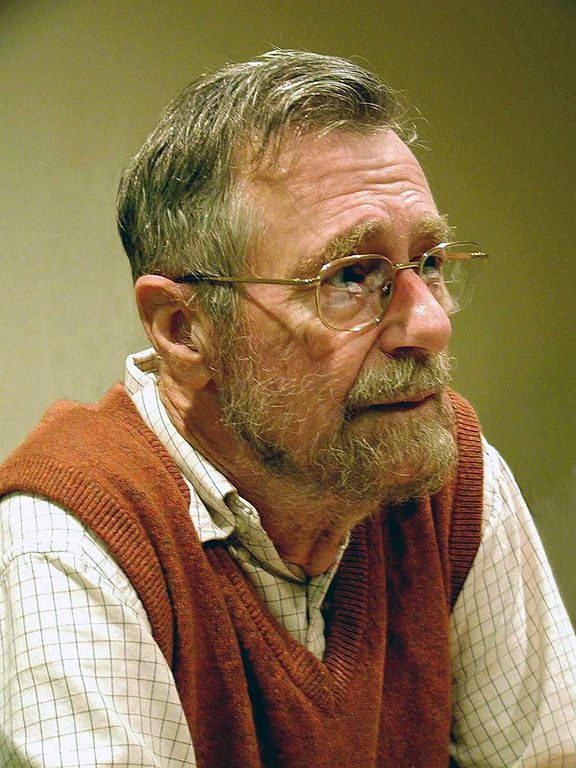
\includegraphics[width=0.75\linewidth]
          {Images/Dijkstra/Edsger_Wybe_Dijkstra.jpg}
        \caption{Portrait \copyright\; Hamilton Richards - manuscripts of
          Edsger W. Dijkstra, University Texas at Austin}
        \label{fig:dijkstra:portrait}
      \end{figure}
    \end{column}
  \end{columns}
\end{frame}